\section{Despliegue}

Para llevar el modelo a producción, se diseñó una arquitectura distribuida basada en contenedores Docker y buenas prácticas de MLOps. A continuación se detalla su estructura:

\subsection{Arquitectura del sistema}
El sistema está organizado en cuatro servicios principales, cada uno desplegado en un contenedor Docker coordinado mediante \texttt{docker-compose}:

\begin{itemize}
  \item \textbf{db}: base de datos MySQL que almacena los experimentos, los metadatos de entrenamiento y los embeddings faciales.
  \item \textbf{mlflow}: servidor de seguimiento MLflow para registrar ejecuciones, métricas, artefactos y modelos entrenados.
  \item \textbf{trainer}: entorno para entrenamiento y pruebas del modelo, incluyendo scripts para generación de experimentos y guardado de modelos.
  \item \textbf{face-api}: API REST basada en \texttt{FastAPI} para ofrecer el servicio de predicción (edad y género) en tiempo real.
\end{itemize}

\subsection{Seguimiento de experimentos y registro de modelos}
Durante la fase de entrenamiento se integró \textbf{MLflow} como plataforma central de seguimiento. Cada ejecución (\textit{run}) dentro del experimento \texttt{AgeGender-UTKFace} registró:

\begin{itemize}
  \item \textbf{Parámetros}: configuración de entrenamiento (número de épocas, tamaño de lote, tasa de aprendizaje).
  \item \textbf{Métricas}: error absoluto medio (MAE) para la predicción de edad y precisión (accuracy) para la clasificación de género, en dos fases distintas (entrenamiento inicial y fine-tuning).
  \item \textbf{Artefactos}: curvas de entrenamiento, matriz de confusión, el modelo exportado en formato TensorFlow y su conversión a ONNX.
\end{itemize}

\begin{figure}[h]
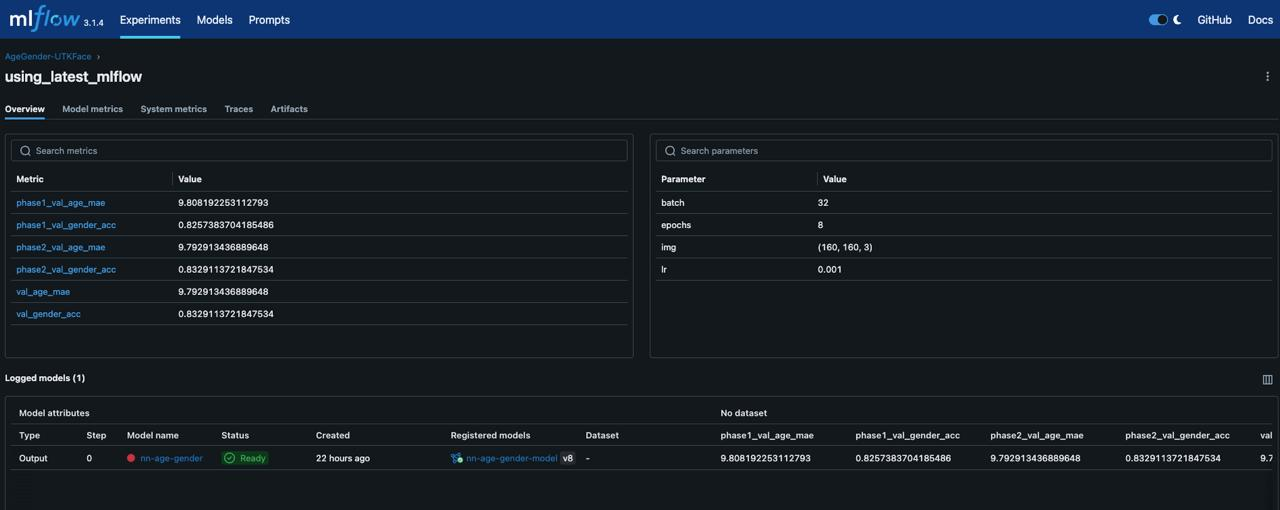
\includegraphics[width=0.5\textwidth]{images/mlflow_metrics.jpeg}
\centering
\caption{Registro de métricas de entrenamiento en MLflow.}
\label{fig:mlflow-metrics}
\end{figure}

\begin{figure}[h]
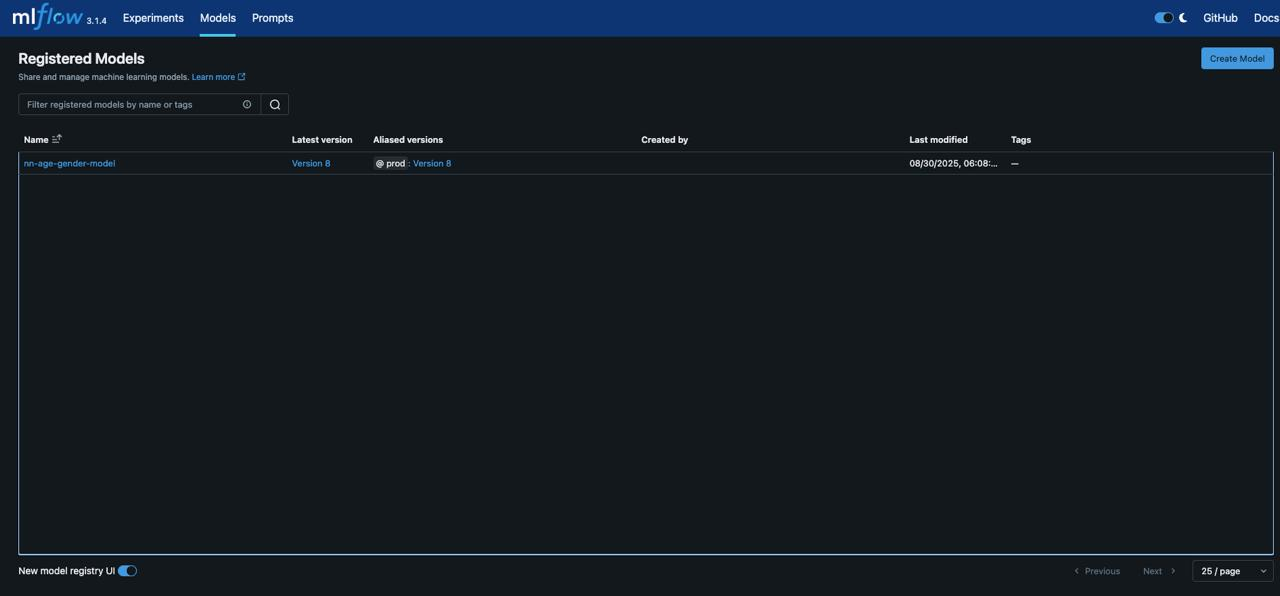
\includegraphics[width=0.5\textwidth]{images/mlflow_register.jpeg}
\centering
\caption{Modelo almacenado en el MLflow Model Registry.}
\label{fig:mlflow-model}
\end{figure}

\subsection{Testing automatizado}
Se incluyó un script de pruebas (\texttt{test\_api.py}) para verificar el correcto funcionamiento de la API (endpoints, respuestas esperadas, formatos JSON, etc.), contribuyendo a garantizar la robustez ante cambios o despliegues posteriores.

\subsection{Contenerización con Docker y orquestación}
Se definió un archivo \texttt{docker-compose.yml} que pone en marcha simultáneamente:
\begin{itemize}
  \item El servicio de base de datos (\texttt{db}),
  \item El servidor MLflow (\texttt{mlflow}),
  \item El entorno de entrenamiento (\texttt{trainer}), y
  \item La API para inferencia (\texttt{face-api}).
\end{itemize}
Esto facilita la configuración, el despliegue en local o en servidor, y la escalabilidad modular del sistema.

\subsection{Carga dinámica de modelos en producción}
Un aspecto clave del despliegue es la \textbf{conexión directa con el MLflow Model Registry}. 
Cuando el contenedor de la API se inicializa, consulta el servidor MLflow definido en la variable de entorno \texttt{MLFLOW\_TRACKING\_URI}. 
Luego solicita la versión del modelo registrada bajo el alias de producción (por ejemplo, \texttt{prod}), descarga ese artefacto y lo carga en memoria para realizar inferencias. 
De esta manera, la API siempre sirve el modelo más reciente validado, sin necesidad de reconstruir la imagen Docker. 
En caso de fallar la conexión, el sistema dispone de mecanismos de respaldo: carga un modelo guardado localmente o, en último recurso, un modelo dummy de prueba.

\subsection{Interfaz de producción: la API REST}
La API permite recibir imágenes, procesarlas (detección, preprocesamiento), ejecutar predicción y devolver los resultados de edad y género. 
Además, puede integrarse fácilmente en aplicaciones externas gracias a su diseño RESTful y a la arquitectura desacoplada.

\begin{figure}[h]
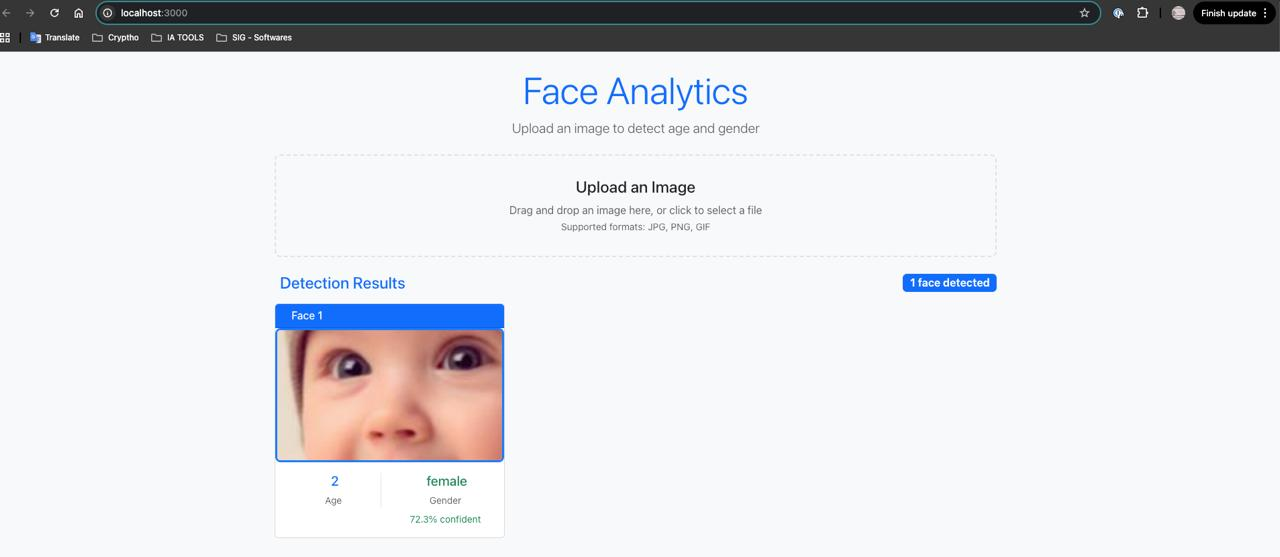
\includegraphics[width=0.5\textwidth]{images/frontend_project.jpeg}
\centering
\caption{Prueba de la API REST con una imagen de entrada y salida de edad/género.}
\label{fig:api-frontend}
\end{figure}

\subsection{Figura ilustrativa del pipeline}
Una figura complementaria (Figura~\ref{fig:deployment-architecture}) representa el flujo completo: 
desde el entrenamiento y registro en MLflow, pasando por la orquestación con Docker, hasta la consulta al Model Registry y la respuesta de predicción servida por la API.

\begin{figure}[h]
\centering
\includegraphics[width=0.5\textwidth]{images/pipeline_workflow.png}
\caption{Pipeline de despliegue: integración entre entrenamiento, MLflow y la API en producción.}
\label{fig:pipeline_workflow}
\end{figure}
